\documentclass{article}
\usepackage[utf8]{inputenc}
\usepackage[spanish]{babel}
\usepackage{listings}
\usepackage{subfigure}
\usepackage{graphicx}
\usepackage{url}
\usepackage{multirow}
\usepackage{color}
\usepackage{booktabs}
\usepackage{float}

\usepackage{hyperref}
\usepackage[margin=3cm,twoside]{geometry} 
\setlength{\parindent}{0pt}
\setlength{\parskip}{1em}


\definecolor{mygreen}{rgb}{0,0.6,0}
\definecolor{mygray}{rgb}{0.5,0.5,0.5}
\definecolor{mymauve}{rgb}{0.58,0,0.82}
\lstset{ 
  backgroundcolor=\color{white},   % choose the background color; you must add \usepackage{color} or \usepackage{xcolor}; should come as last argument
  basicstyle=\footnotesize,        % the size of the fonts that are used for the code
  breakatwhitespace=false,         % sets if automatic breaks should only happen at whitespace
  breaklines=true,                 % sets automatic line breaking
  captionpos=b,                    % sets the caption-position to bottom
  commentstyle=\color{mygreen},    % comment style
  deletekeywords={...},            % if you want to delete keywords from the given language
  escapeinside={\%}{)},          % if you want to add LaTeX within your code
  extendedchars=true,              % lets you use non-ASCII characters; for 8-bits encodings only, does not work with UTF-8
  firstnumber=1,                % start line enumeration with line 1000
  frame=single,	                   % adds a frame around the code
  keepspaces=true,                 % keeps spaces in text, useful for keeping indentation of code (possibly needs columns=flexible)
  keywordstyle=\color{blue},       % keyword style
  language=Octave,                 % the language of the code
  morekeywords={*,...},            % if you want to add more keywords to the set
  numbers=left,                    % where to put the line-numbers; possible values are (none, left, right)
  numbersep=5pt,                   % how far the line-numbers are from the code
  numberstyle=\tiny\color{mygray}, % the style that is used for the line-numbers
  rulecolor=\color{black},         % if not set, the frame-color may be changed on line-breaks within not-black text (e.g. comments (green here))
  showspaces=false,                % show spaces everywhere adding particular underscores; it overrides 'showstringspaces'
  showstringspaces=false,          % underline spaces within strings only
  showtabs=false,                  % show tabs within strings adding particular underscores
  stepnumber=1,                    % the step between two line-numbers. If it's 1, each line will be numbered
  stringstyle=\color{mymauve},     % string literal style
  tabsize=2,	                   % sets default tabsize to 2 spaces
  title=\lstname                  % show the filename of files included with \lstinputlisting; also try caption instead of title
}
\usepackage{etoolbox}
\makeatletter
\providecommand{\subtitle}[1]{% add subtitle to \maketitle
  \apptocmd{\@title}{\par {\large #1 \par}}{}{}
}
\makeatother
\title{Tarea 3 de Modelos Probabilistas Aplicados}
\subtitle{Distribuciones de Probabilidad}

\author{5271}
\date{\today}

\begin{document}

\maketitle

\section{Origen de los datos}

En este trabajo se utiliza como fuente de los datos el libro ``The Adventures of Sherlock Holmes" \cite{Holmes92}, del escritor y médico británico Arthur Conan Doyle. Este libro se encuentra disponible en la biblioteca virtual gratuita Project Gutenberg, con el siguiente enlace: \href{https://www.gutenberg.org}{https://www.gutenberg.org}. 

\section{Sobre el libro}

Este libro es una colección de doce cuentos de Arthur Conan Doyle, los cuales fueron publicados por primera vez el 14 de octubre de 1892. El mismo agrupa los primeros cuentos con el detective consultor Sherlock Holmes, que se habían publicado en doce números mensuales de The Strand Magazine de Julio de 1891 a junio de 1892. 

\section{Análisis y tratamiento de los datos}

Al libro seleccionado se le realiza un estudio de frecuencia de ocurrencia de la cantidad de letras por palabras, de palabras por oraciones y cantidad de oraciones por párrafo. El análisis será realizado en el programa R versión 4.0.2 \cite{r} en el entorno de desarrollo Rstudio \cite{rstudio}. 

\subsection{Letras por oraciones}
De le libro en cuestión se extraen todas las palabras que componen el texto, de las mismas se eliminan la llamadas palabras ``vacías", es decir las que no aportan contenido al libro, el resultado del filtro se muestra en el cuadro \ref{tab:1} de la página \pageref{tab:1}. Una vez realizado este filtrado se procede a contar la cantidad de letras que tiene cada palabra, como se observa en la figura \ref{fig:1}(a) de la página \pageref{fig:a}. En la figura \ref{fig:1}(b) de la página \pageref{fig:b}, se muestra la distribución binomial negativa con parámetros $n = $ cantidad de palabras después del filtro, $k = 18$ y $p = 0.75 $, a la que se asemeja la distribución de las cantidad de letras por palabras en el texto analizado.

% Table generated by Excel2LaTeX from sheet 'palabrasvacias'
\begin{table}
  \centering
  \caption{fragmento de \textit{Data frame} resultante del filtrado}
    \begin{tabular}{rrl}
    \toprule
          & \multicolumn{1}{l}{\textbf{Gutenberg\_id}} & \textbf{Palabras} \\
    \midrule
    2     & 1661  & sherlock \\
    3     & 1661  & holmes \\
    19    & 1661  & mystery \\
    20    & 1661  & orange \\
    167   & 1661  & crime \\
    168   & 1661  & occupied \\
    169   & 1661  & immense \\
    170   & 1661  & faculties \\
    171   & 1661  & extraordinary \\
    172   & 1661  & powers \\
    \bottomrule
    \end{tabular}%
  \label{tab:1}%
\end{table}%

\begin{figure}
\centering
\subfigure[Cantidad de letras por palabras]{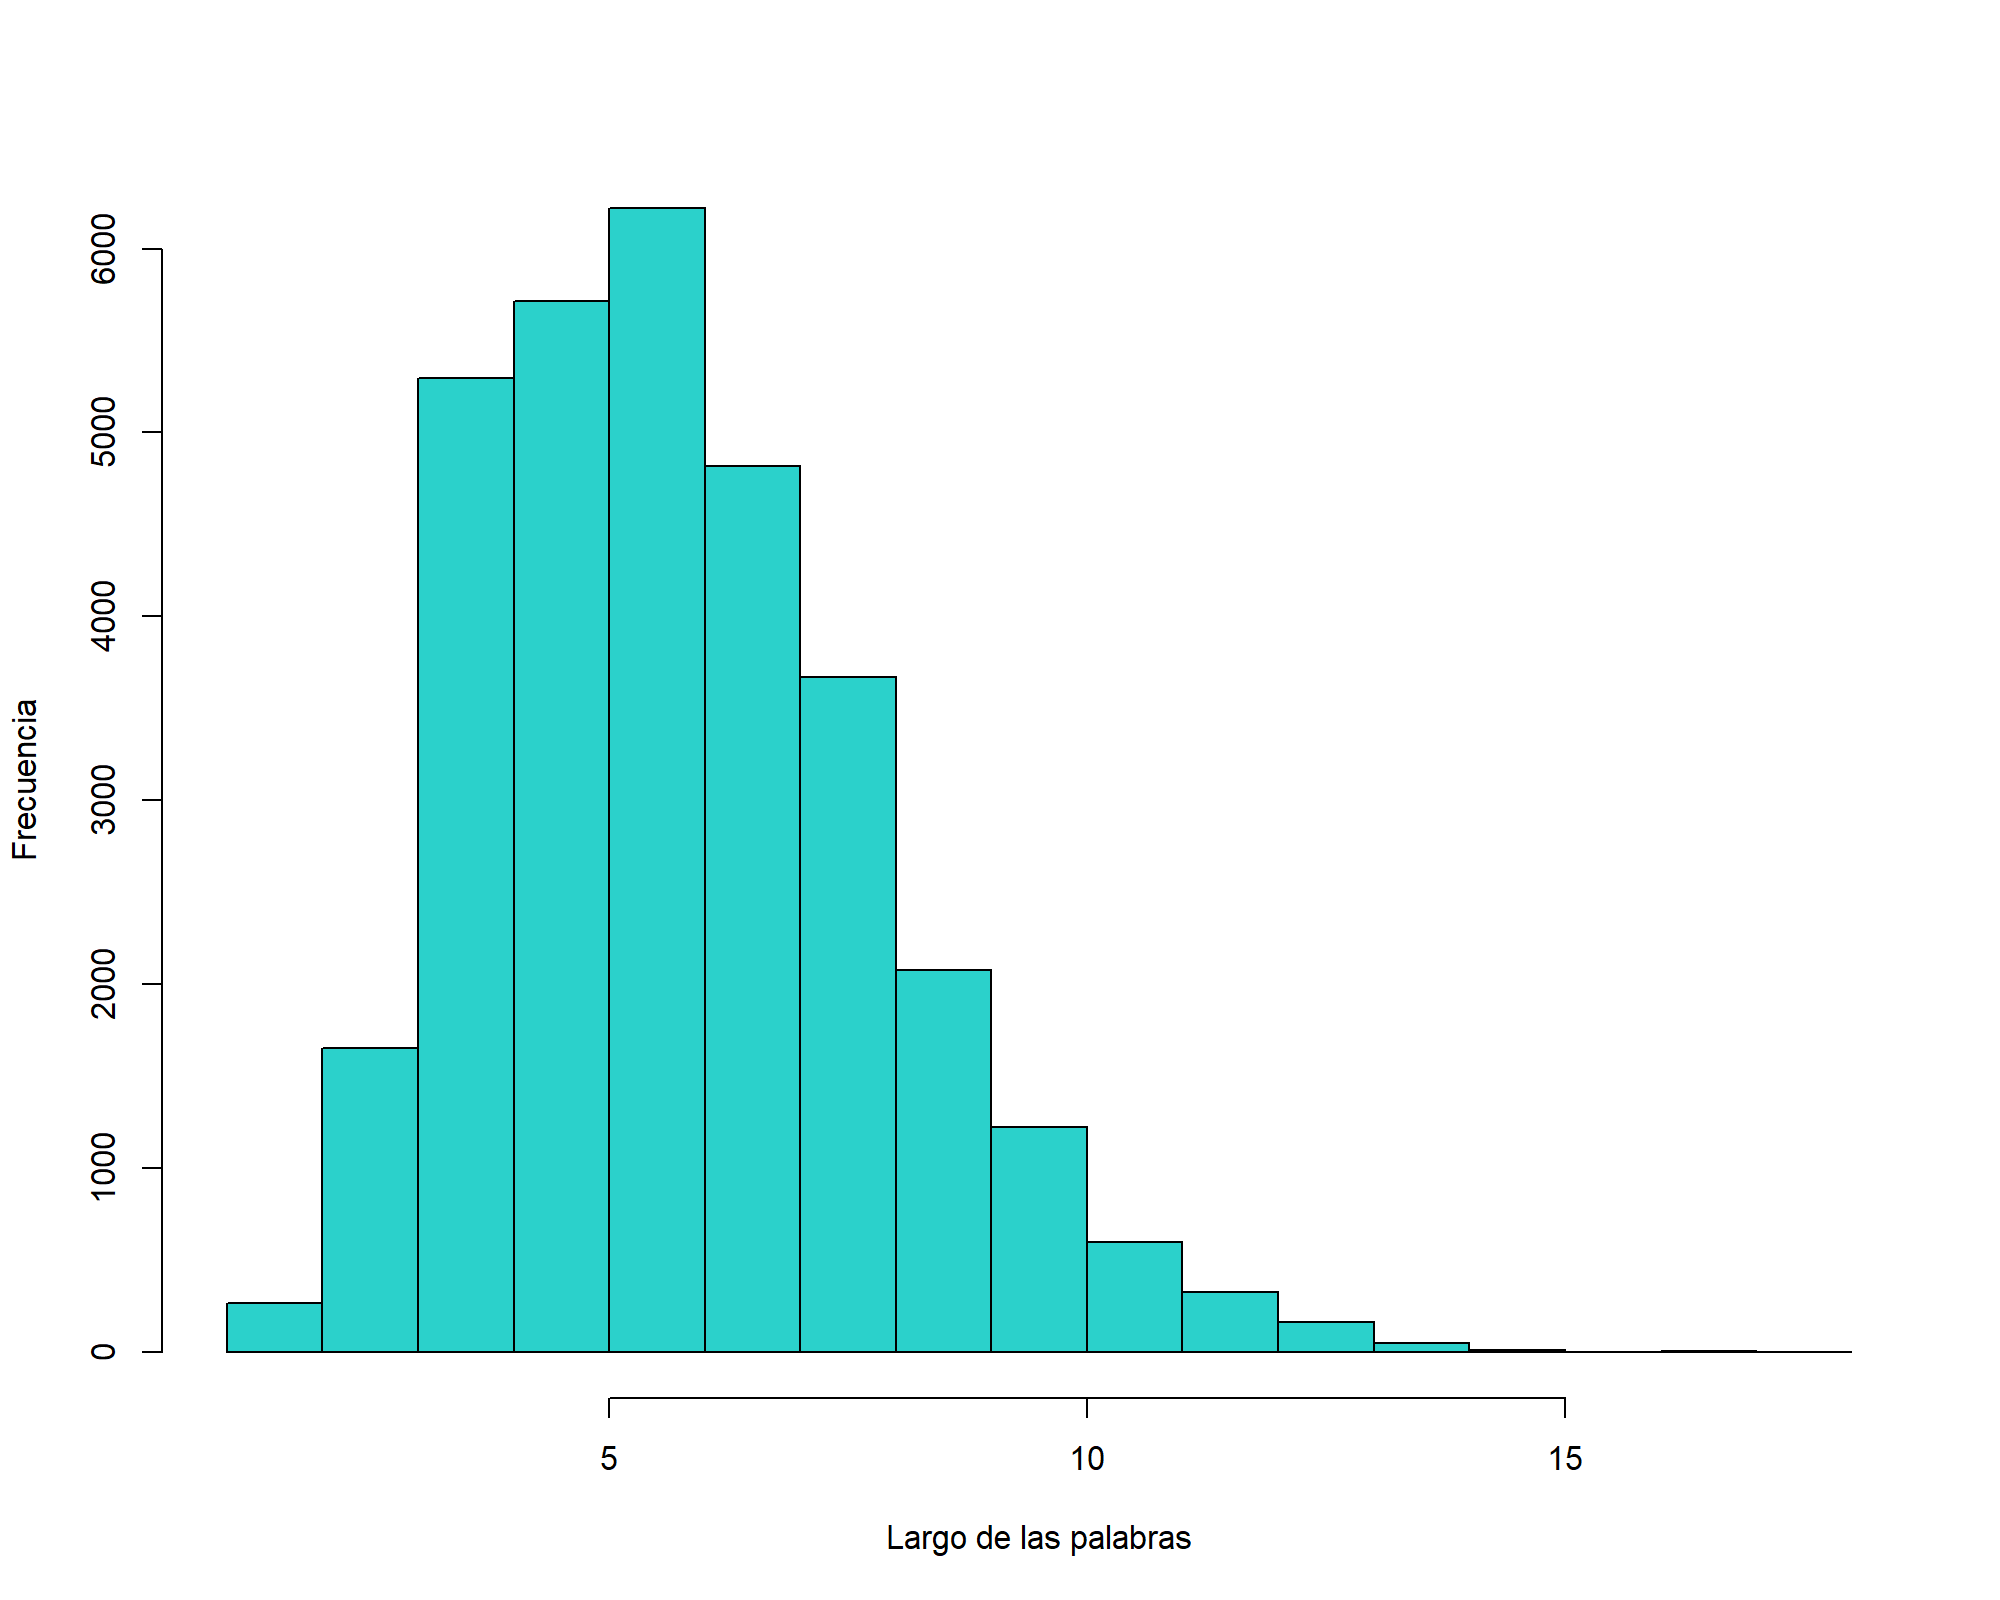
\includegraphics[scale=0.5]{figuras/frecuenciacantletras.png}}
\label{fig:a}
\centering
\subfigure[distribución binomial negativa creada con la función \textit{rnbinom} de R ]{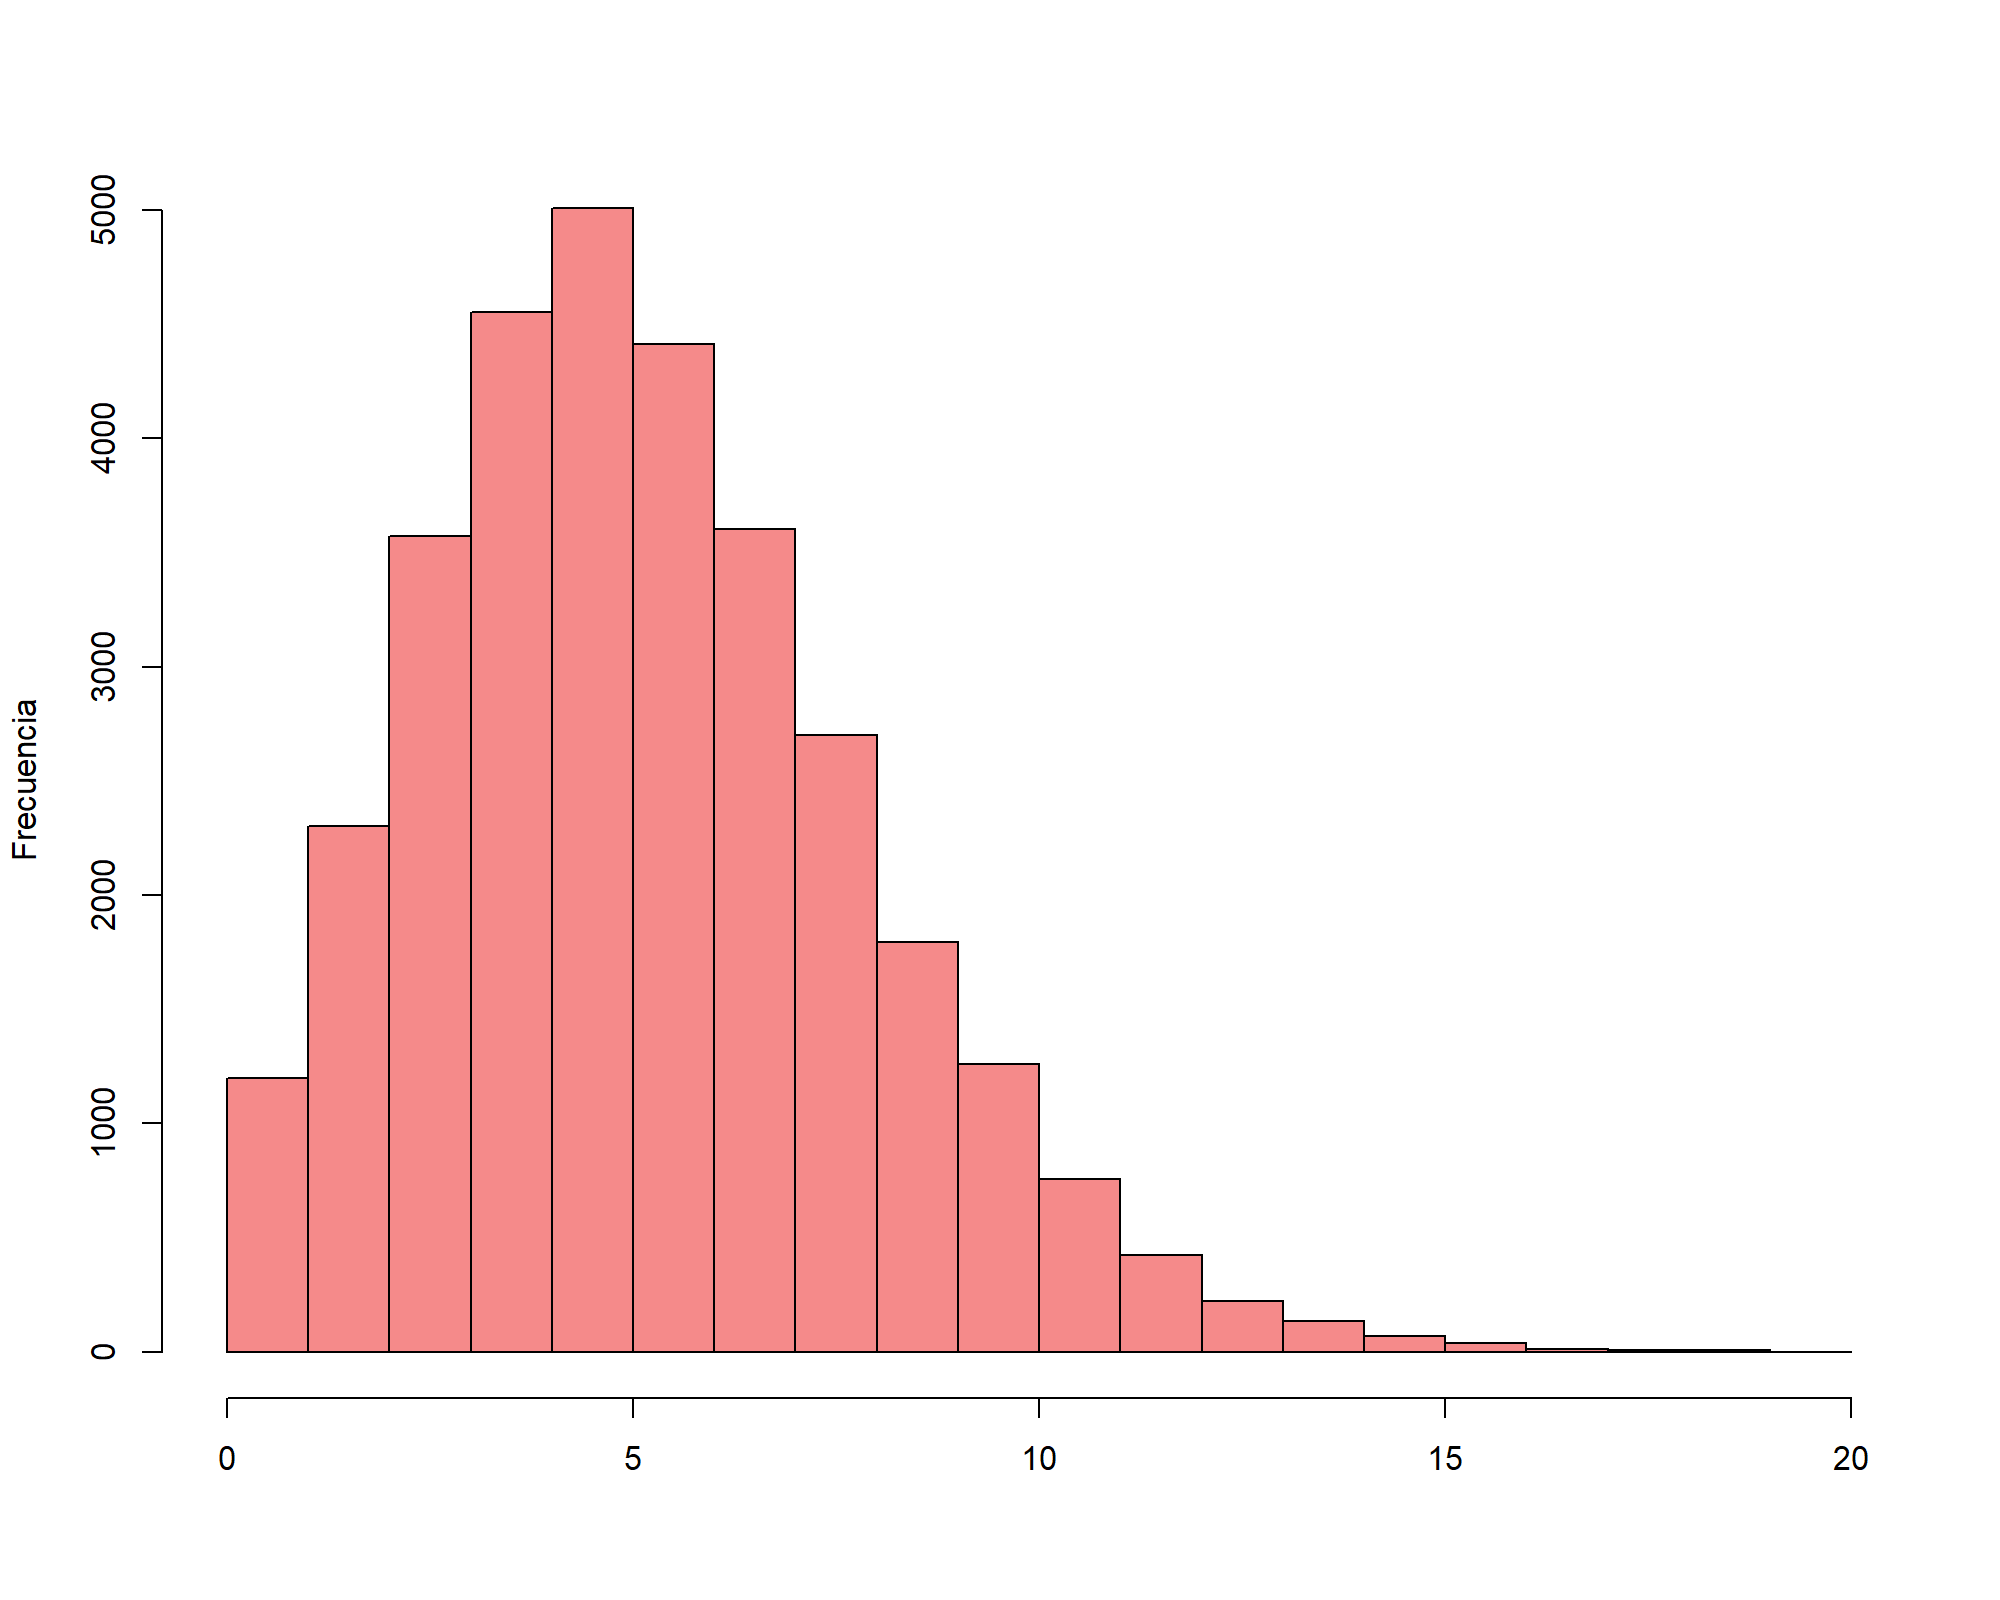
\includegraphics[scale=0.5]{figuras/nbinom.png}}
\label{fig:b}
\vspace{-0.2cm}
\caption{Histogramas de distribución de cuantiad de letras por palabras en el texto}
\label{fig:1} 
\end{figure}


 \subsection{Palabras por oraciones}
  Para el trabajo con las oraciones, se extraen todas las presentes en el texto y se cuenta la cantidad de palabras que conforman cada una de estas oraciones. Lo anterior se puede observar en la en la figura \ref{fig:2}(a) de la página \pageref{fig:2}. En la figura \ref{fig:2}(b) de la página \pageref{fig:2} se muestra una distribución geométrica con parámetros $n =$ cantidad de oraciones del texto y $p = 0.055$. Dicha distribución se asemeja a la distribución de la cantidad de palabras en las oraciones del texto.
 
 
\begin{figure}
\centering
\subfigure[Cantidad de palabras por oraciones]{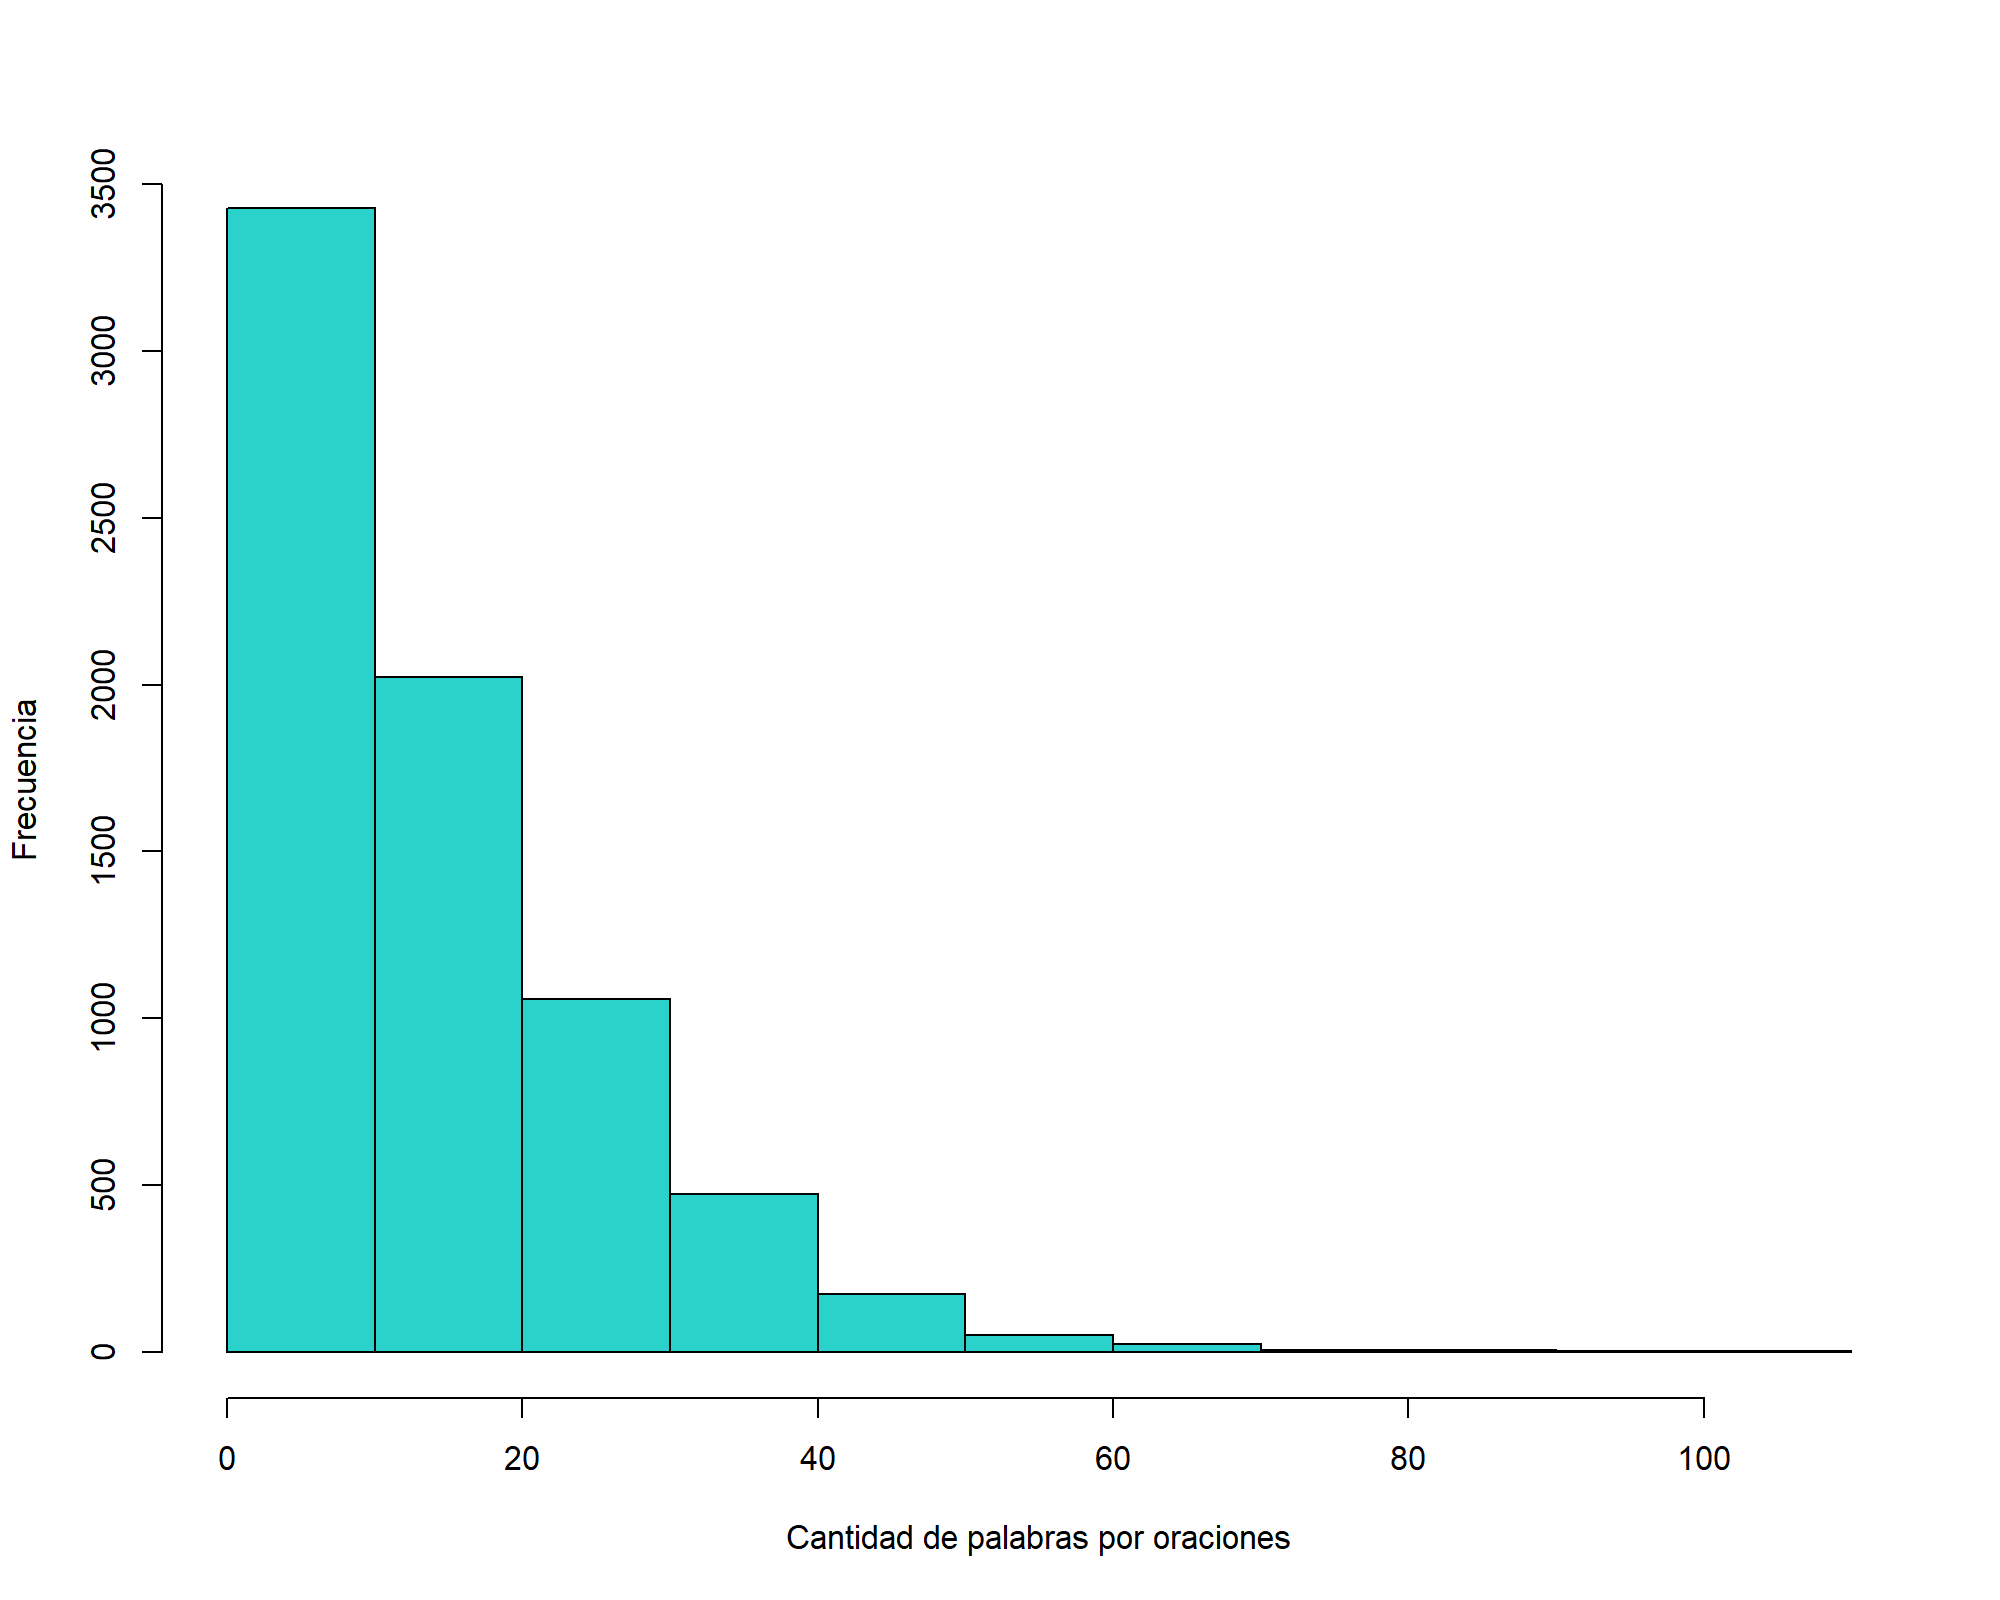
\includegraphics[scale=0.5]{figuras/frecuenciapalabras3.png}}
\label{fig:a}
\centering
\subfigure[distribución geométrica creada con la función \textit{rgeom} de R ]{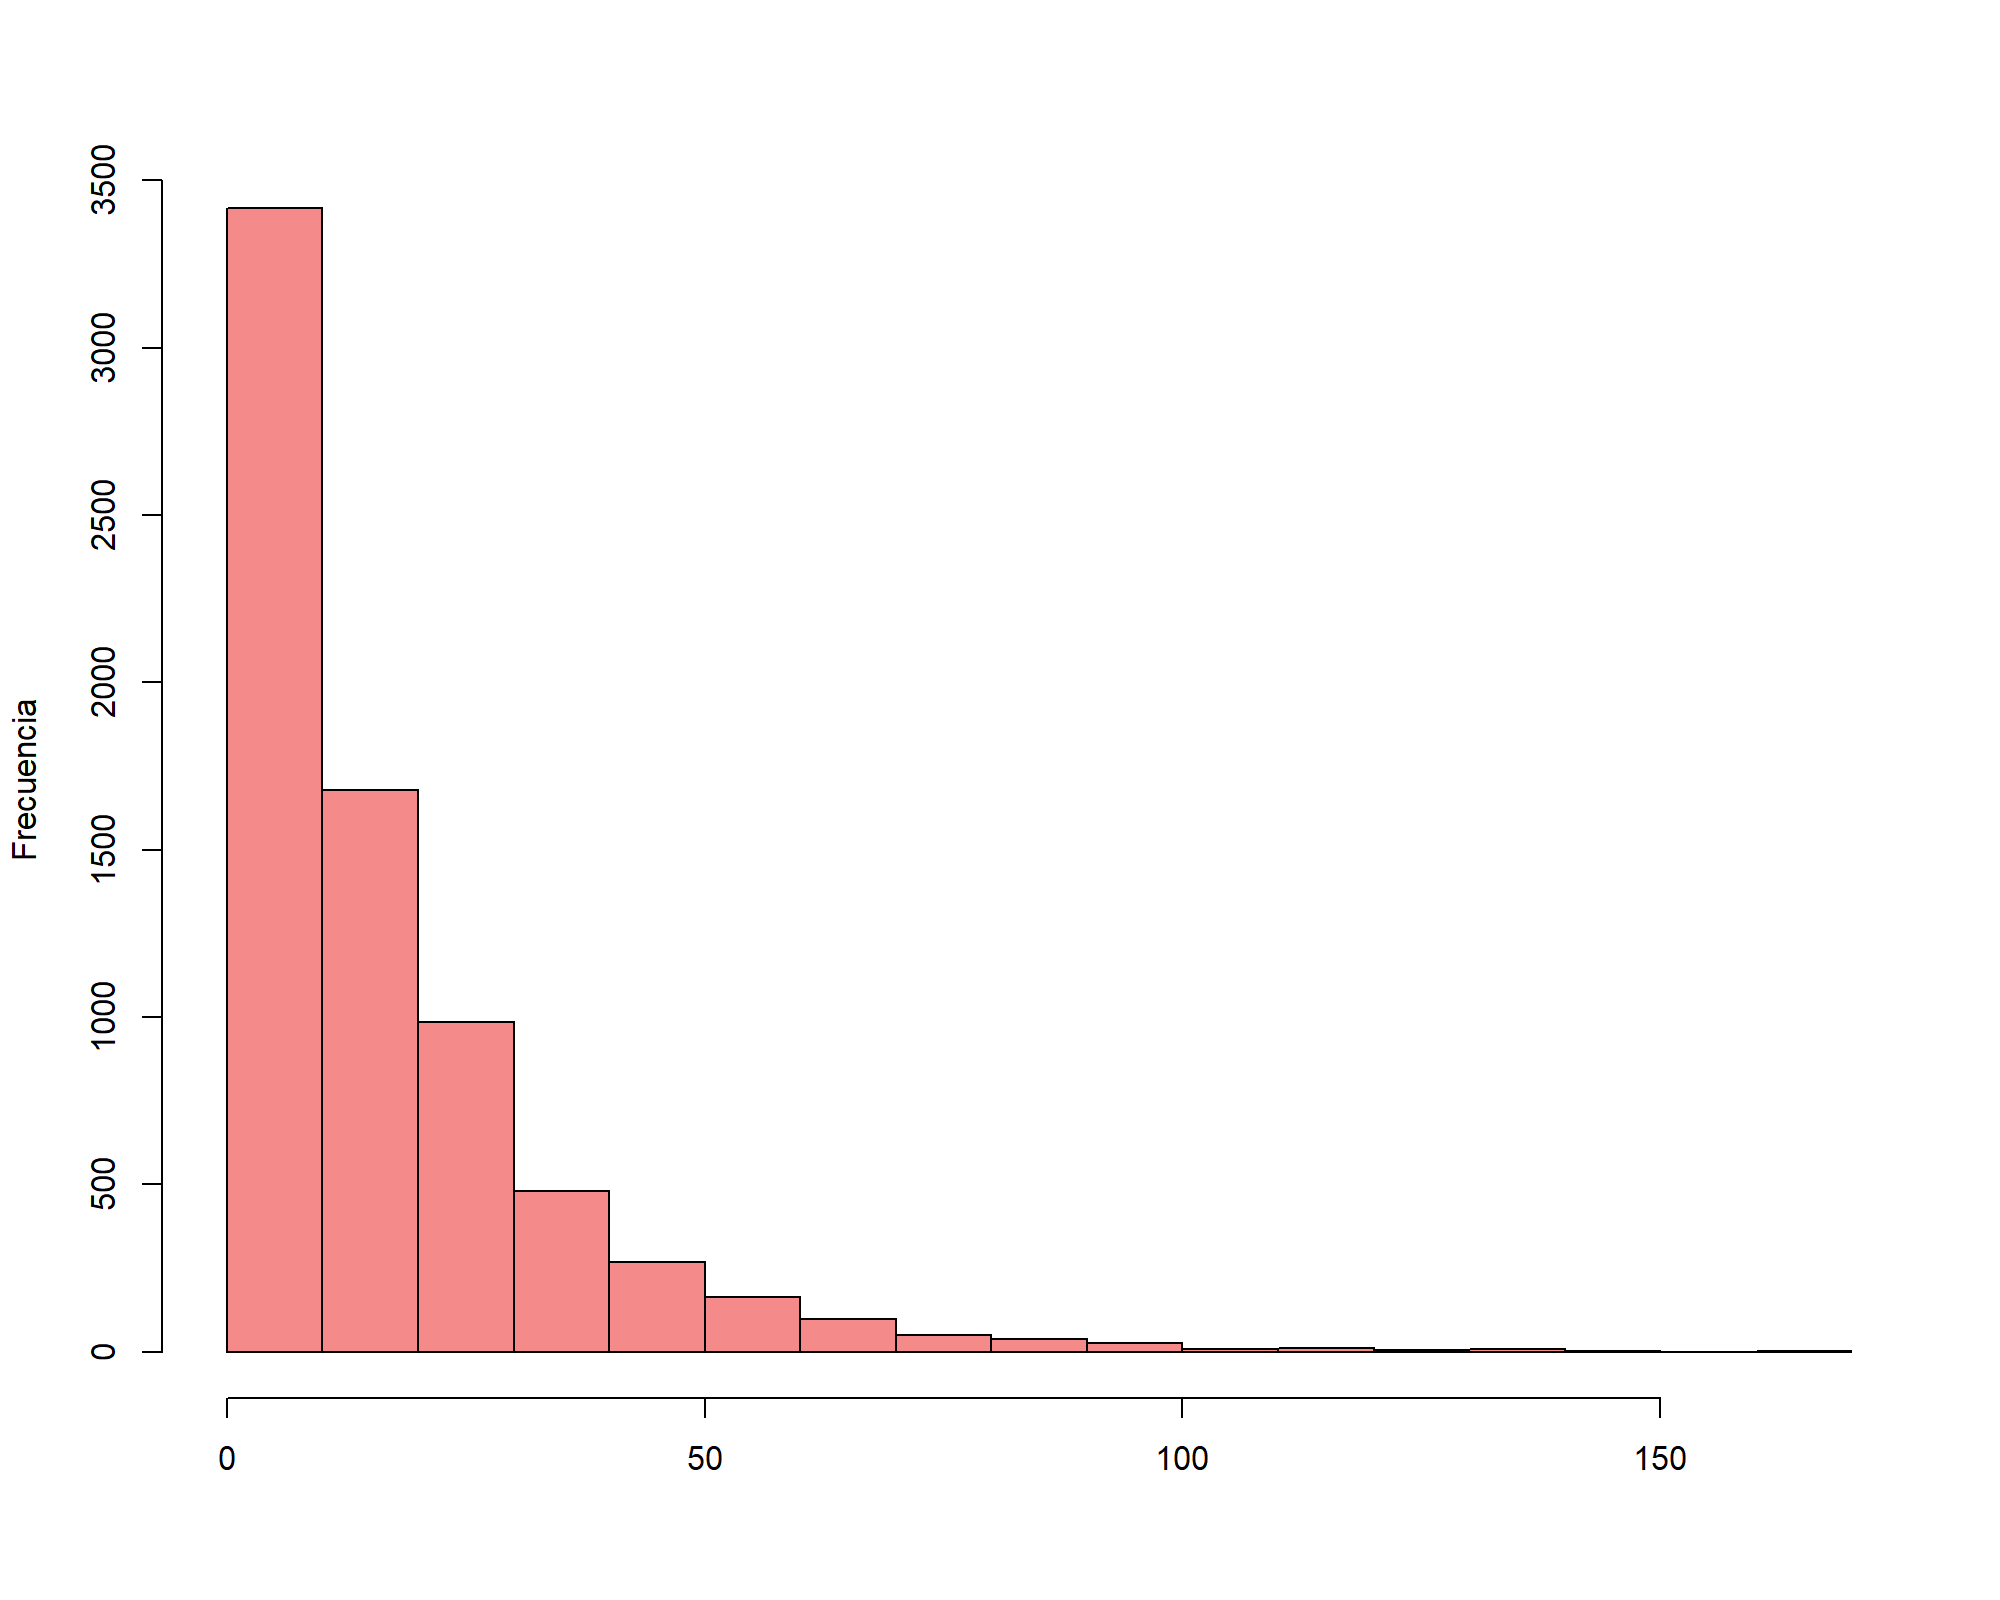
\includegraphics[scale=0.5]{figuras/geometrica.png}}
\label{fig:b}
\vspace{-0.2cm}
\caption{Histogramas de distribución de cuantiad de palabras por oraciones en el texto}
\label{fig:2} 
\end{figure}
 
 \subsection{Oraciones por párrafos}
Análogamente a lo realizado en la subsecciones anteriores se procede al análisis de la cantidad de oraciones por párrafo, como se puede observar en la figura \ref{fig:3}(a) de la página \pageref{fig:3}. En la figura \ref{fig:3}(b) de la página \pageref{fig:3} se muestra una distribución geométrica con parámetros $n =$ cantidad de párrafos del texto y $p = 0.29 $. La distribución mostrada en figura \ref{fig:3}(b) es muy similar a la distribución de la cantidad de oraciones por párrafos en el libro.
 
\begin{figure}
\centering
\subfigure[Cantidad de oraciones por párrafos]{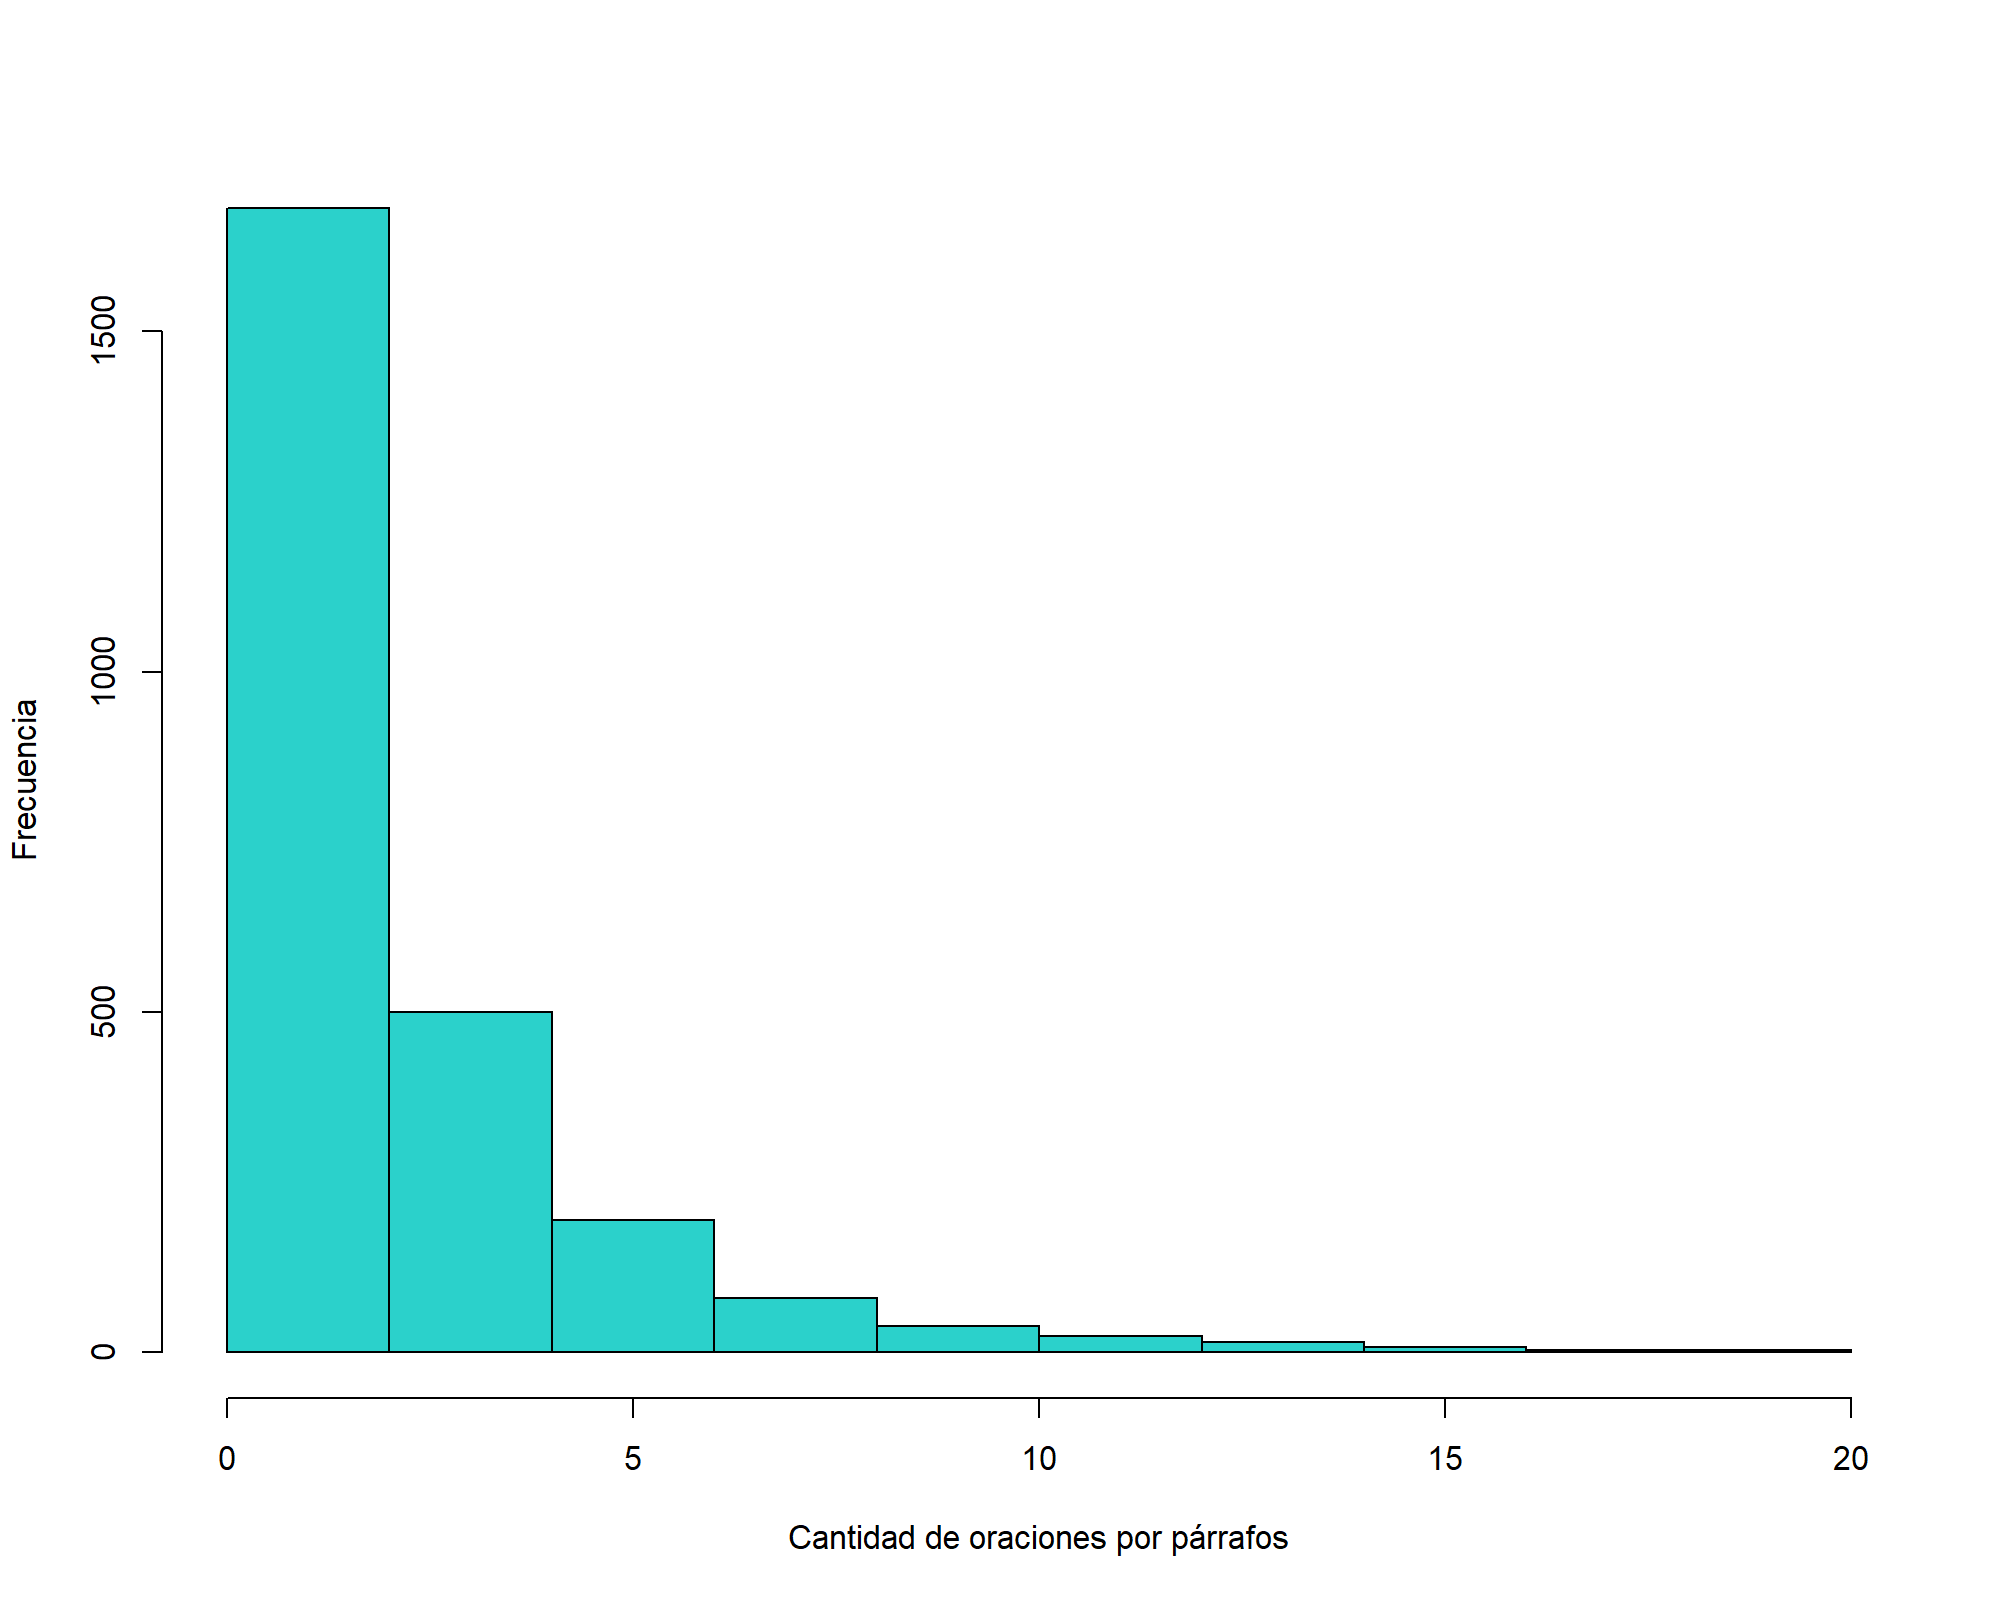
\includegraphics[scale=0.5]{figuras/frecuenciaoraciones.png}}
\label{fig:a}
\centering
\subfigure[distribución geométrica creada con la función \textit{rgeom} de R ]{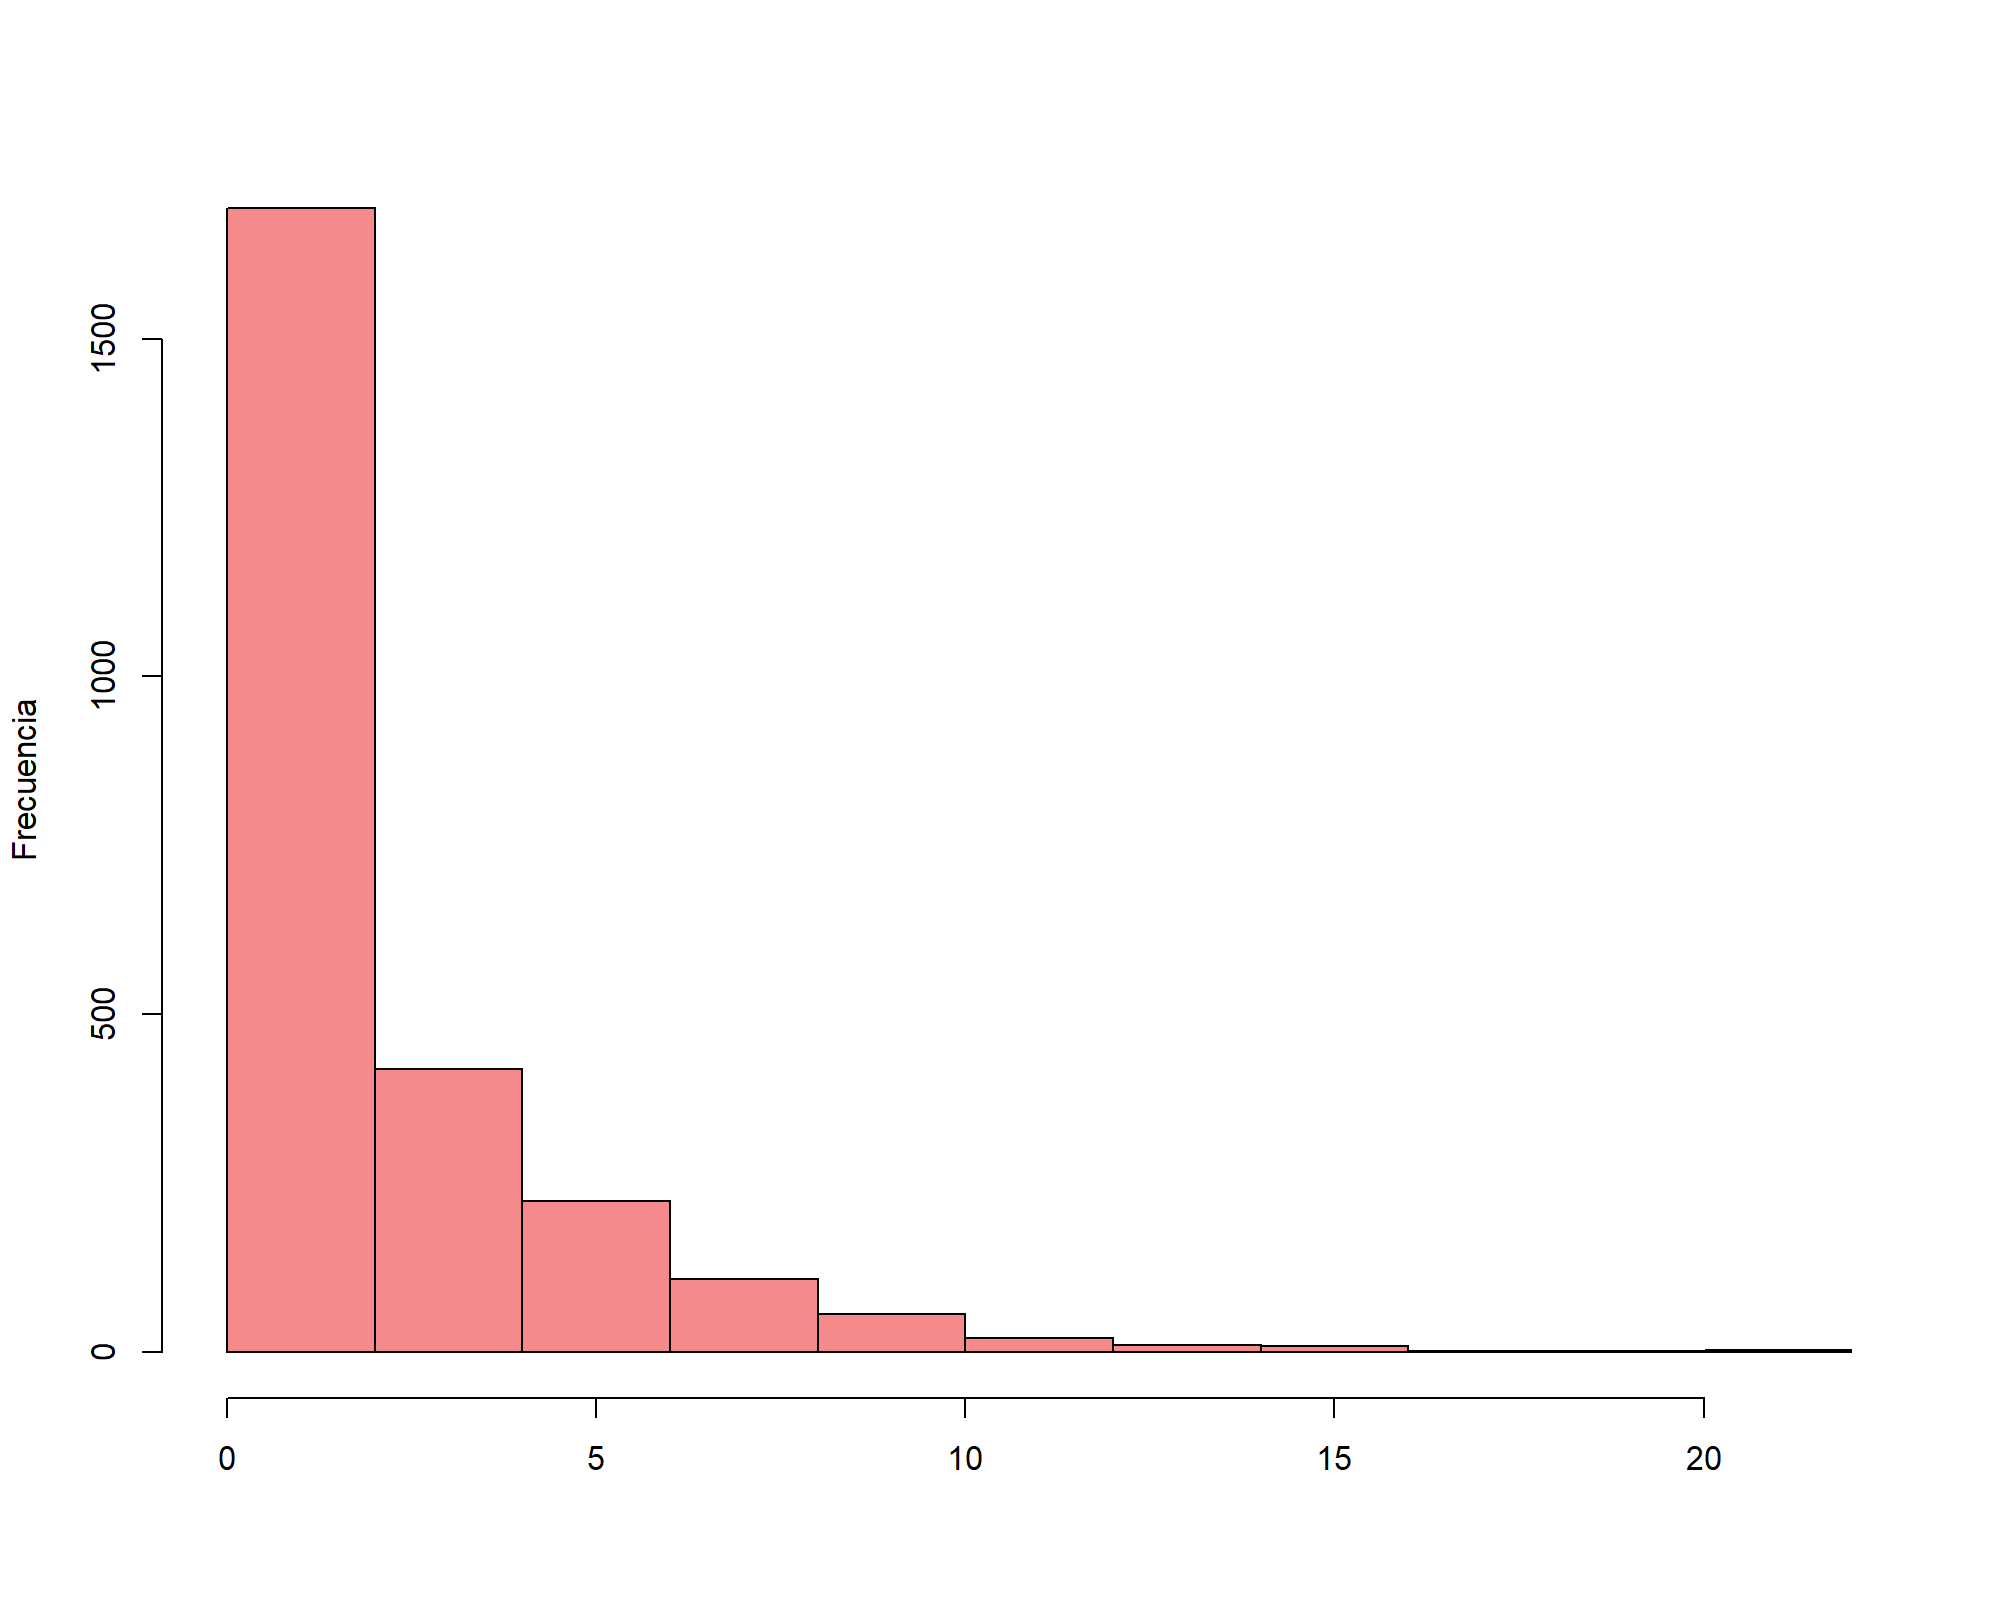
\includegraphics[scale=0.5]{figuras/geometricaparafo.png}}
\label{fig:b}
\vspace{-0.2cm}
\caption{Histogramas de distribución de cuantiad de oraciones por párrafos en el libro}
\label{fig:3} 
\end{figure}

El código general se encuentra disponible en el repositorio \href{https://github.com/Albertomnoa/Tareas_MPA/tree/master/Tarea3}{https://github.com/Albertomnoa/Tareas} 

\newpage
\bibliographystyle{plain}
\bibliography{Biblio}

\end{document}
